\documentclass[a4paper]{article}
\usepackage[margin=0.5in]{geometry}
\usepackage[T1]{fontenc}
\usepackage[utf8]{inputenc}
\usepackage{lmodern}
\usepackage{amsmath}
\usepackage{amssymb}
\usepackage{geometry}
\usepackage{enumerate}
\usepackage{xcolor}
\usepackage{graphicx}
\usepackage{amsthm}
\newtheorem{theorem}{Theorem}[section]
\newtheorem{lemma}[theorem]{Lemma}
\newtheorem{corollary}[theorem]{Corollary}
\newtheorem{definition}[theorem]{Definition}
\usepackage{listings}
\usepackage{authblk}
\usepackage{titling}
\usepackage{zlmtt}
\usepackage{fancyvrb}
\usepackage[hidelinks]{hyperref}
\setlength{\droptitle}{-2em}
\lstset{frame=tb,
  language=C,
  aboveskip=3mm,
  belowskip=3mm,
  showstringspaces=false,   
  columns=flexible,
  basicstyle={\small\ttfamily},
  numbers=none,
  numberstyle=\tiny\color{gray},
  keywordstyle=\color{blue},
  commentstyle=\color{brown},
  stringstyle=\color{orange},
  breaklines=true,
  breakatwhitespace=true,
  tabsize=3
}
\begin{document}
\title{CS3210 Lab 2 Report}
\author{
  Wang Xiyu (A0282500R),\\ Sun Weiyang (A0287903U) (Discussed with)
}
\maketitle
\section*{Ex11}
\subsection*{Instruction per Cycle}
\par\vspace{3ex}
\begin{minipage}{0.5\linewidth}
    \noindent\makebox[\columnwidth][c]{%
        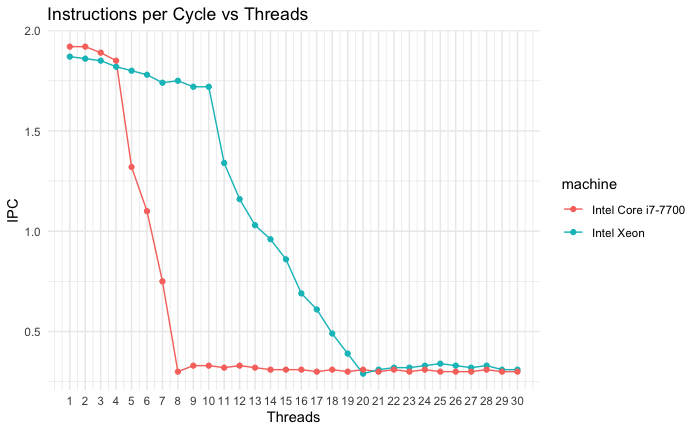
\includegraphics[
        width=\columnwidth,
        clip
        ]{ipc.png}
    }
\end{minipage}\hfill
\begin{minipage}{0.4\linewidth}
    
\end{minipage}\hfill
\subsection*{Wall clock time}
\begin{minipage}{0.5\linewidth}
    \noindent\makebox[\columnwidth][c]{%
  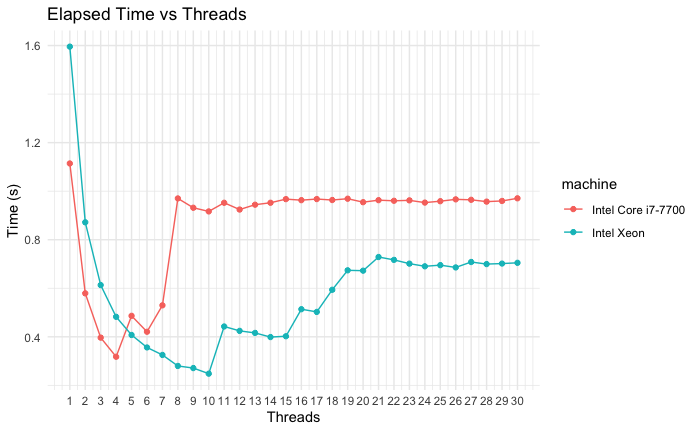
\includegraphics[
    width=\columnwidth,
    trim=0 0 0 0,
    clip
  ]{time.png}
}
\end{minipage}\hfill
\begin{minipage}{0.4\linewidth}
aaa
\end{minipage}\hfill
\par\vspace{3ex}
\subsection*{MFLOPS}
\begin{minipage}{0.5\linewidth}
    \noindent\makebox[\columnwidth][c]{%
    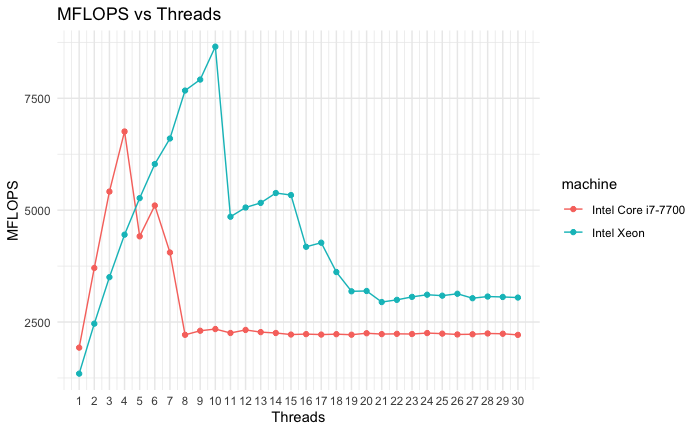
\includegraphics[
      width=\columnwidth,
      trim=0 0 0 0,
      clip
    ]{mflops.png}
    }
\end{minipage}\hfill
\begin{minipage}{0.4\linewidth}
aaa
\end{minipage}\hfill





\end{document}